\newpage

\section{Návrh}

Na základe analýzy problémovej oblasti a existujúcich riešení sme sa rozhodli najprv použiť konvolučnú neurónovú sieť (jej popis a architektúra v kapitole \ref{nn_popis}), čo sa pretavilo aj do prvotných experimentov (kapitola \ref{first_experiments}) vykonávaných v rámci predmetu Počítačové videnie\footnote{http://vgg.fiit.stuba.sk/teaching/computer-vision/}.

\subsection{Návrh neurónovej siete}
\label{nn_popis}

Celá architektúra je načrtnutá na schéme na obrázku \ref{my_tensorboard_cnn} vytvorenej pomocou nástroja  TensorBoard\footnote{https://www.tensorflow.org/get\_started/summaries\_and\_tensorboard/}.

Jedná sa o jednoduchú sieť so vstupnou konvolučnou vrstvou pre spracovanie obrázkov. Táto vrstva obsahuje konvolučný filter (veľkosť \textit{5x5}) s aktivačnou funkciou sigmoid. Výstup z nej ďalej pokračuje do vrstvy združovania, kde sa použije operácia MAX s filtrom o veľkosti \textit{2x2} a krokom tiež s veľkosťou \textit{2}. Po nich nasleduje vrstva normalizácie, kde je celý výstup zlúčený do jednej širokej vrstvy. Za ňou sa nachádza plne prepojená vrstva (z angl. fully-connected layer) s aktivačnou funkciou sigmoid a vrstva výpadku (z angl. dropout layer\cite{dropout}), ktorej hodnota (v rozmedzí od 0 do 1) určuje, aké percentuálne množstvo neurónov aj s prepojeniami bude dočasne skrytých. Táto možnosť umožňuje počas učenia sa predchádzať pretrénovaniu. Za vrstvou výpadku už nasleduje iba výstupná vrstva a jej transformácia na 2D maticu, obrázok predstavujúci mapu výraznosti, ktorú chceme dostať.

Aktivačná funkcia sigmoid je použitá najmä preto, že mapa výraznosti je prakticky pravdepodobnostné rozdelenie, t. j. sieť sa snaží predikovať pravdepodobnosti výraznosti každého pixelu. Ako algoritmus učenia sme zvolili štandardný algoritmus spätného šírenia chyby (z angl. backpropagation) s trochu extravagatným FTRL optimizérom.

\begin{figure}[H]
	\begin{center}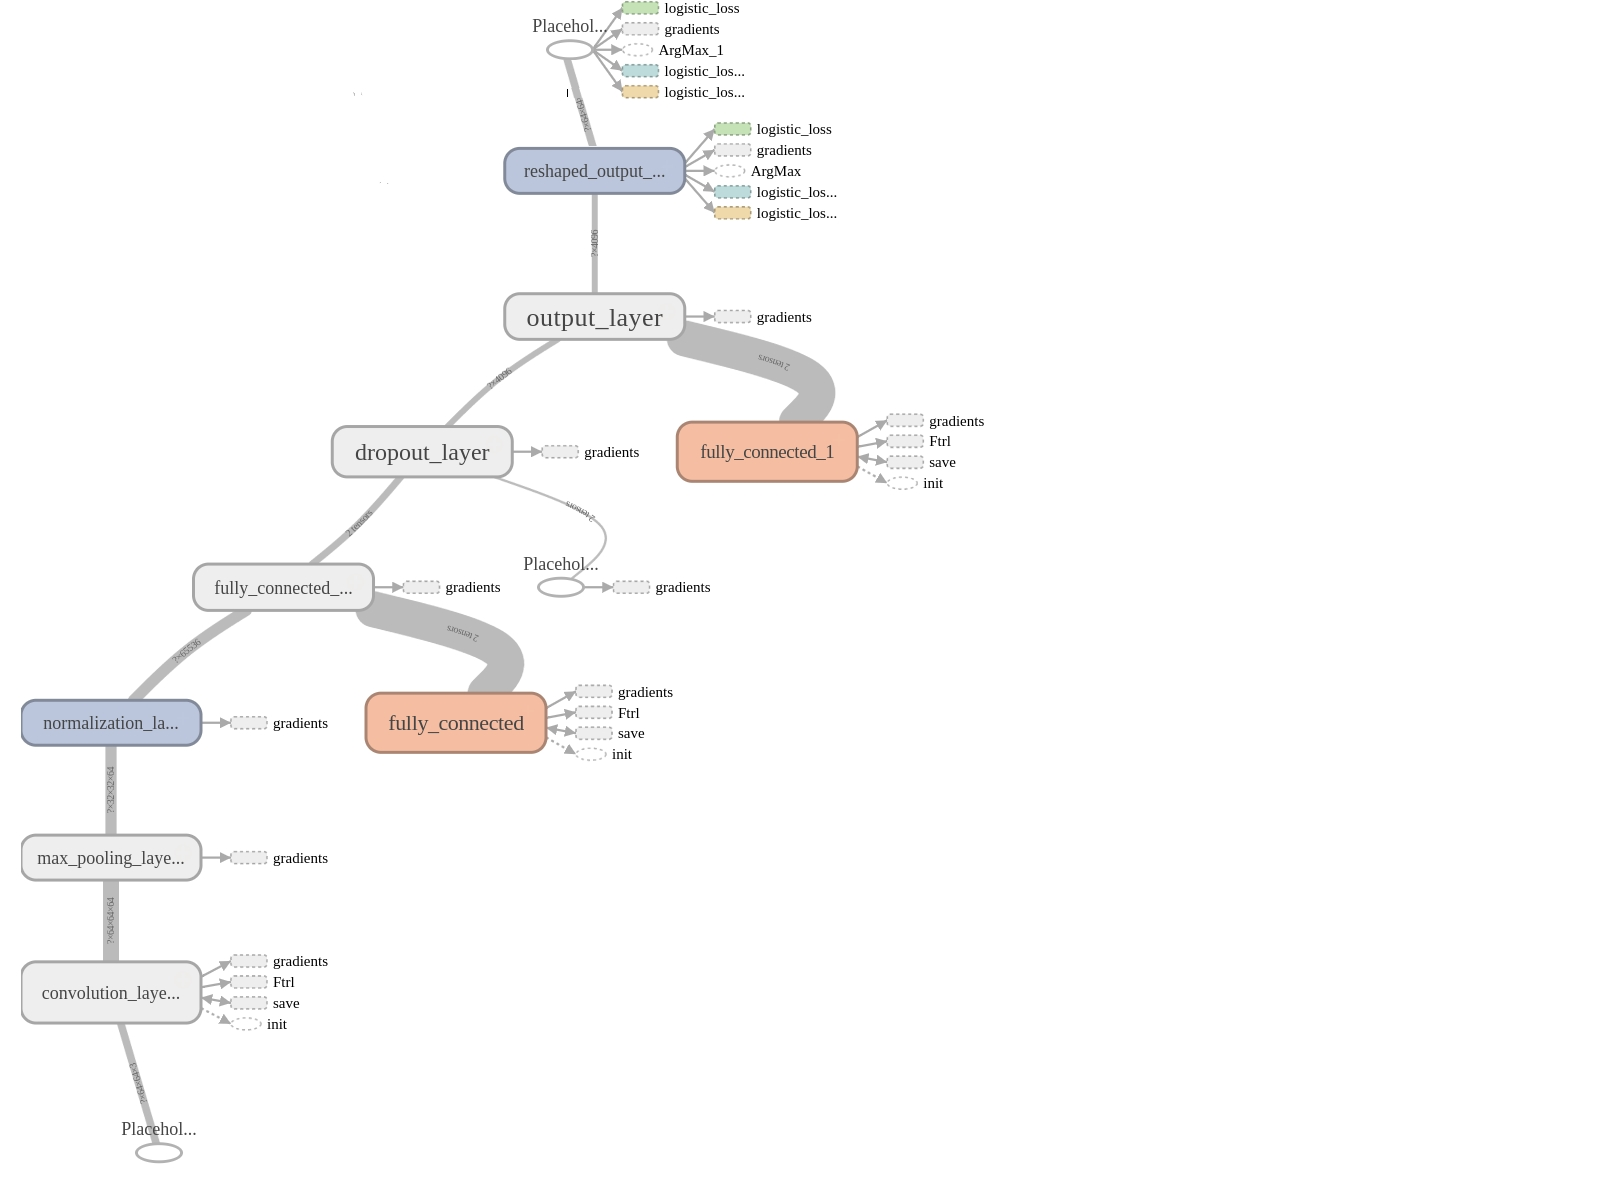
\includegraphics[scale=0.4]{graph-run.jpg}
		\caption[Návrh architektúry neurónovej siete]{
			Diagram reprezentujúci architektúru neurónovej siete, zdola vstupná konvolučná vrstva nasledovaná ostatnými vrstvami siete až po výstupnú, spolu s transformáciou na 2D maticu reprezentujúcu predikovanú mapu výraznosti pre vstupný obrázok
		}\label{my_tensorboard_cnn}
	\end{center}
\end{figure}

\subsection{Prvotné experimenty}
\label{first_experiments}
Pre prvotné experimenty sme sa rozhodli zvoliť problém predikcie vizuálnej pozornosti v častiach obrázkov, konkrétne v tzv. regiónoch záujmu (z angl. regions of interest, ROIs), ktoré sme zvolili v okolí fixácií na obrázky. Z veľkého množstva problémov, s ktorými sme sa potýkali, bol jedným z najväčších práve dataset, keďže bolo nutné vhodne ho zvoliť a predpripraviť (extrakcia regionóv záujmu pre obrázky, mapy výraznosti, správne oštítkovanie, ...)

\subsubsection{Dataset}
\label{dataset}
Dataset použitý k trénovaniu navrhnutej neurónovej siete tvorili spomínané regióny zájmu extrahované z niekoľkých voľne dostupných dataset-ov vizuálnej pozornosti (CAT2000\cite{borji2015cat2000}, NUSEF\footnote{http://mmas.comp.nus.edu.sg/NUSEF.html}, ...). Keďže vo viacerých z nich chýbali úplné informácie k výpočtu máp výraznosti, rozhodli sme sa ich extrahovať rovnako ako pri obrázkoch scény z obrázkov máp výraznosti. Vizualizáciu popisovanej extrakcie v okolí fixácií možno vidieť na obrázku \ref{roi_image}. Nevyhovujúce časti datasetov (ako napr. abstraktné umienie, fraktály, cartoon obrázky, ...) boli odfiltrované.

\begin{figure}[H]
	\begin{center}
		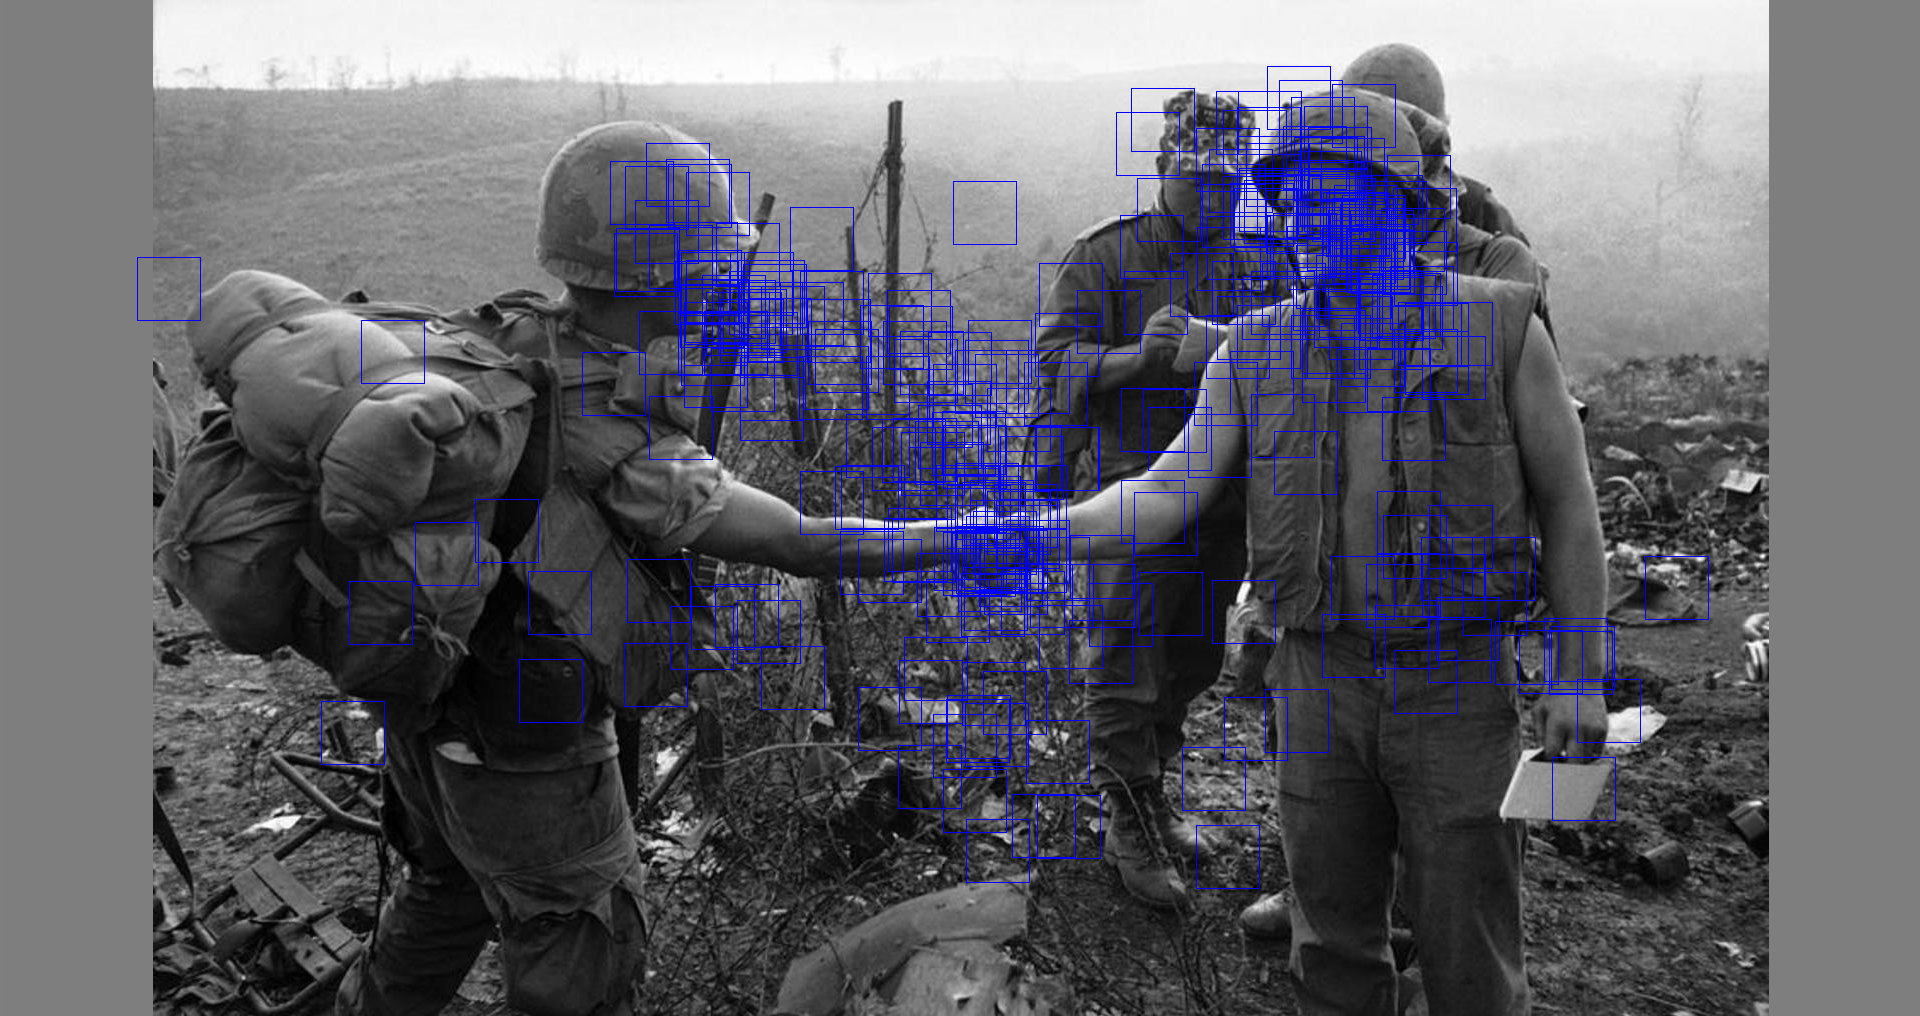
\includegraphics[scale=0.13]{img.png}
		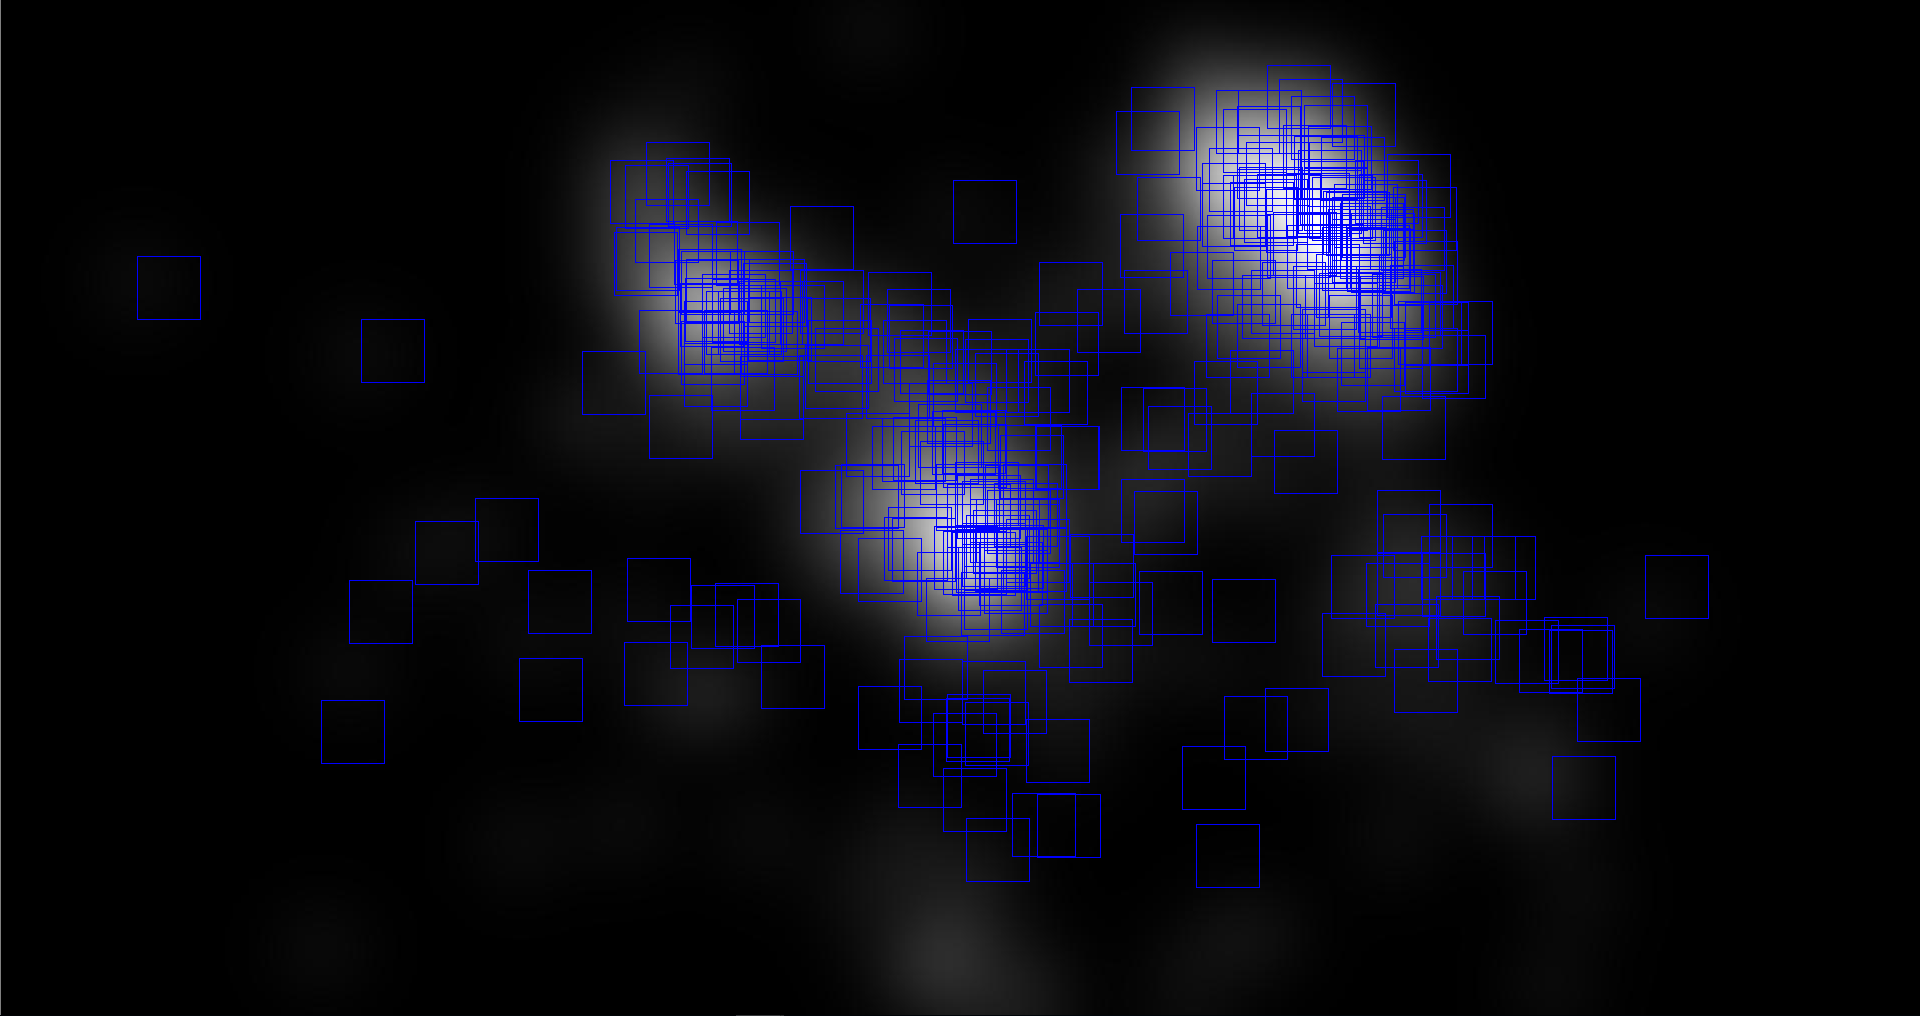
\includegraphics[scale=0.13]{map.png}
		\caption[Vizualizácia extrakcie regiónov záujmu]{
			Vizualizácia extrakcie regiónov záujmu, vľavo obrázok, vpravo mapa výraznosti k nemu
		}\label{roi_image}
	\end{center}
\end{figure}

Mapy výraznosti boli extrahované ako grayscale obrázky, kde hodnota pixelu prakticky určuje intenzitu. Získané dáta boli ďalej pre neurónovú sieť normalizované.
\newline

\subsubsection{Výsledky}

Navrhovanú sieť sme trénovali na priravenom datasete (nakoniec obsahoval zhruba 500 000 vzoriek), ktorý bol rozdelený štandardne v pomere 80:10:10 (80 - trénovanie, 10 - validácia, 10 - testovanie). Validácia prebiehala po každej iterácii a trénovanie končilo v momente keď sa chyba na validačných dátach začala výrazne odlišovať oproti najnižšej dosiahnutej (pomaly dochádzalo k pretrénovaniu). V závere mala sieť chybu predikcie na testovacích dátach na úrovni \textit{0.29}, chyba bola počítaná ako priemer chýb v každom bode obrázka. Na obrázku \ref{results_image} možno vidieť porovanie predikovaných máp výraznosti s originálnymi a so vstupnými obrázkami. 

\begin{figure}[H]
	\begin{center}
		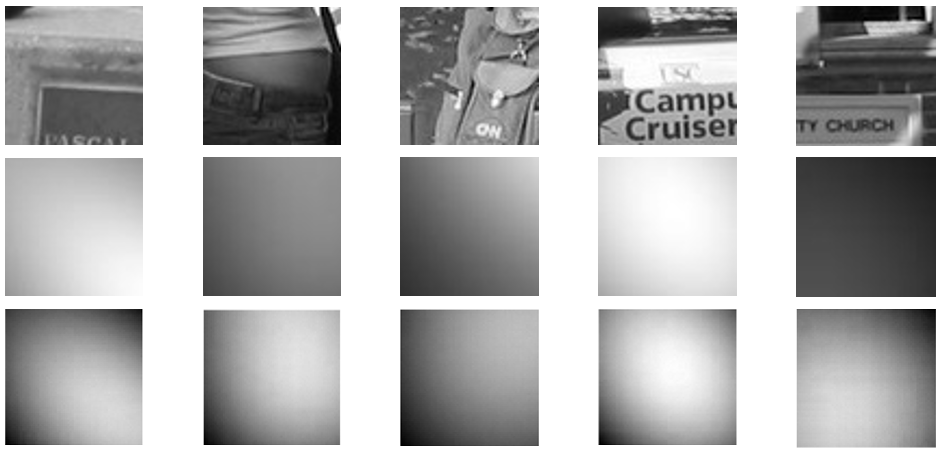
\includegraphics[scale=0.5]{predicted_saliency.png}
		\caption[Porovnanie prvotných výsledkov]{
			Porovnanie predikcií (dolu) s originálnymi mapami výraznosti (v strede) voči vstupným obrázkom (hore)
		}\label{results_image}
	\end{center}
\end{figure}

Pri snahe vypočítať metriky pre predikcie sme narazili na problém, ktorý sme si na začiatku neuvedomili. Väčšina metrík evaluuje mapu výraznosti voči binárnej matici reprezentujúcej fixácie na obrázok. Vzhľadom na to, že našim vstupom boli regióny záujmy v okolí fixácií, vo väčšine prípadov tieto binárne matice obsahovali len jednu fixáciu. Vďaka tomu mali metriky (AUC, sAUC, NSS) nezmyselne vysoké hodnoty. Z tohto dôvodu ich teda považujeme za nerelevantné a jediná metrika, podľa ktorej sa môžeme riadiť, je korelačný koeficient, keďže ten evaluuje predikovanú mapu voči tej pôvodnej. Jeho hodnoty na testovacích dátach sa v priemere pohybovali na hranici 0.563.